% !TEX root =  ../main_manuscript.tex 
\section{Application of Personalized Schedules in Prostate Cancer Surveillance}
\label{sec:results}
We next demonstrate personalized schedules for scheduling biopsies in prostate cancer active surveillance. To this end, we reuse results from a joint model we previously fitted~\citep{tomer2019personalized} to the PRIAS dataset introduced in Section~\ref{sec:introduction}. This model utilized a linear mixed sub-model for biannually measured PSA (continuous: log-transformed from ng/mL), and a logistic mixed sub-model for biannually measured DRE (binary: tumor palpable or not). The model employed B-splines~\citep{de1978practical} to accommodate non-linear PSA evolution over follow-up. In the survival sub-model, fitted PSA value, fitted instantaneous PSA velocity (defined in Section~\ref{subsec:surival_sub_model}), and log-odds of having a DRE indicating a palpable tumor, were included as time-dependent predictors. The model parameters were estimated under the Bayesian framework~\citep{tomer2019personalized} using the R package \textbf{JMbayes}~\citep{rizopoulosJMbayes}. While the complete model definition and parameter estimates are provided in~\citet{tomer2019personalized}, we next briefly present the key results relevant for personalized scheduling.

First, the cause-specific cumulative-risk of cancer progression at the maximum study period of ten years was 50\% (Web-Figure~1). This indicates that many patients may not require all of the yearly biopsies they are usually prescribed. Since personalized schedules are risk-based, their overall performance is dependent on the predictive accuracy and discrimination capacity of the fitted model. In this regard, the model had a moderate area under the receiver operating characteristic curve (AUC) over the follow-up period (between 0.61 and 0.68). The mean absolute prediction error was moderate to large (between 0.08 and 0.24) and decreased rapidly after year one of the follow-up. Thus, personalized schedules based on this model may work better after year one with more follow-up data.

\subsection{Personalized Biopsy Schedules for a Demonstration Prostate Cancer Patient}
\label{subsec:demo_patient}
We utilized the joint model fitted to the PRIAS dataset to schedule biopsies in a demonstration prostate cancer patient shown in Figure~\ref{fig:demo_schedule}. The time of his last negative biopsy was $t=3.5$ years, and the time of the current visit was $v=5$ years. We made biopsy decisions over his future visits for PSA measurement $U=\{u_1=5, u_2=5.5,\ldots,u_L=10\}$ years using four different schedules. Two of the fixed schedules are annual biopsy schedule and the PRIAS schedule. The PRIAS schedule has compulsory biopsies at year one, four, seven, and ten of follow-up, and additional annual biopsies if PSA doubling-time~\citep{bokhorst2015compliance} is high. Remaining two schedules are personalized, namely, with a fixed threshold $\kappa=10\%$ risk, and an automatically chosen current visit time $v$ specific risk $\kappa^*(v)$ (Section~\ref{subsec:kappa_selection}). Since the demonstration patient's time of last negative biopsy $t=3.5$ is after year one of follow-up, a time delay in detecting progression
up to three years may not lead to adverse downstream outcomes~\citep{carvalho}.

\begin{figure}
\centerline{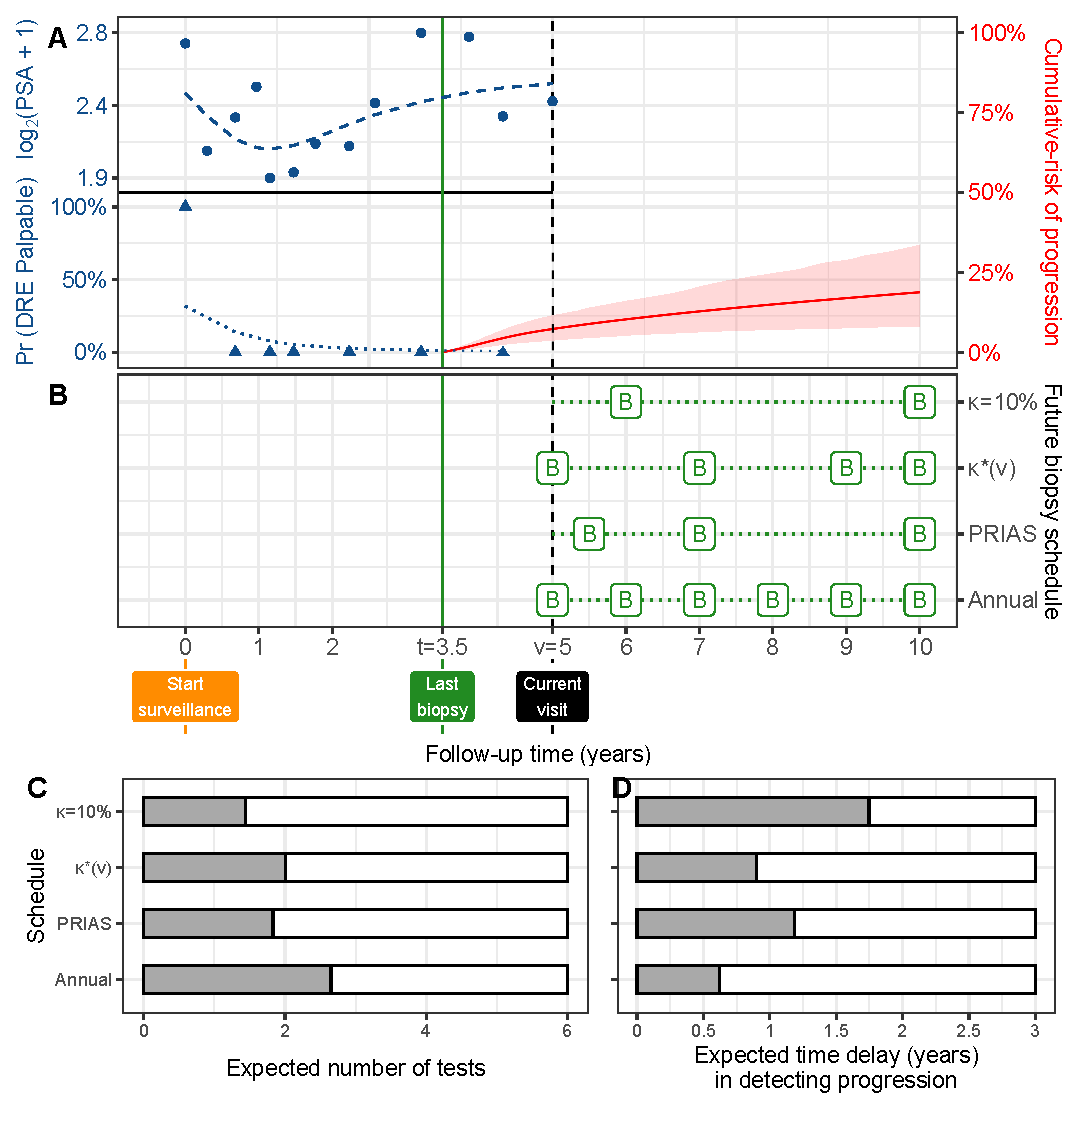
\includegraphics{images/demo_schedule.eps}}
\caption{\textbf{Personalized schedules for a demonstration prostate cancer patient}. \textbf{Panel~A}: Time of current visit: $v=5$ years (black dashed line). Time of last negative biopsy: $t=3.5$ years (vertical green solid line). Longitudinal data: $\log_2(\mbox{PSA} + 1)$ transformed~\citep{tomer2019personalized} PSA (observed: blue dots, fitted: dashed blue line), and binary DRE (observed: blue triangles, fitted probability: dotted blue line). Cumulative-risk profile: solid red line (95\% credible interval shaded). \textbf{Panel~B}: Different biopsy schedules are shown with a `B' indicating a biopsy. \textbf{$\kappa=10\%$} and \textbf{$\kappa^*(v)$} are personalized biopsy schedules using a risk threshold of 10\%, and a visit time $v$ specific automatically chosen threshold~(\ref{eq:kappa_choice}), respectively. PRIAS and Annual denote the PRIAS biopsy schedule (Section~\ref{subsec:demo_patient}) and annual biopsy schedule. \textbf{Panel~C,D}: For all schedules we calculate the expected number of tests and expected time delay in detecting progression if the patient progresses before year ten. Since a recommended minimum gap of one year is maintained between biopsies, maximum possible number of tests are six. A delay in detecting progression of up to three years may not lead to adverse outcomes~\citep{carvalho}. }
\label{fig:demo_schedule}
\end{figure}

The cumulative-risk of progression of the demonstration patient increases 3\% yearly on average, up to 19\% at the maximum study period of ten years. Hence, the patient may progress slowly. Consequently, risk-based personalized approaches plan fewer biopsies than the annual schedule (Panel~B, Figure~\ref{fig:demo_schedule}). Also, the time delay in detecting progression for personalized schedules (Panel~D, Figure~\ref{fig:demo_schedule}) is below the safe limit of three years mentioned earlier. Thus, personalized schedules can be a suitable alternative to the annual schedule.

\subsection{Web-application for Personalized Biopsy Schedules Prostate Cancer Surveillance}
We implemented the methodology for scheduling risk-based biopsies in prostate cancer active surveillance in a web-application (\url{https://emcbiostatistics.shinyapps.io/prias\_biopsy\_recommender/}). In this web-application, four types of risk-based personalized schedules are provided, namely, using 5\%, 10\%, and 15\% fixed thresholds, and a current-visit time specific optimal threshold obtained via~(\ref{eq:kappa_choice}). Also, a general purpose source code for creating personalized test schedules is provided in Web-Appendix~D. The source code is compatible with joint models fitted using the R package \textbf{JMbayes}~\citep{rizopoulosJMbayes}.